\documentclass[12pt]{article}
\usepackage[english]{babel}
\usepackage{url}
\usepackage{graphicx}
\usepackage{indentfirst}
\usepackage{microtype}
\usepackage{float}

\graphicspath{ {./figures/} }


\begin{document}

\begin{titlepage}
	\begin{center}
		\vspace*{1cm}

		{\fontsize{17}{16}\selectfont \textbf{PE35 - UPorto NFC Virtual Card}}


		\vspace{0.5cm}
		Final Report of Projeto Integrador

		\vspace{1.5cm}

		\textbf{António Henrique Martins Azevedo}\\
		\textbf{António Marujo Rama}\\
		\textbf{Francisco Miguel Correia Mariano Pinheiro Cardoso}\\
		\textbf{Tomás Eiras Silva Martins}\\

		\vfill

		
\includegraphics[width=0.4\textwidth]{UPORTO_fundotransparente}

		\vfill

		Licenciatura em Engenharia Informática e Computação

		\vspace{0.8cm}

		\textbf{Tutor in U.Porto}: Pedro Miguel Alves Brandão\\
		\textbf{Proponent}: Rodolfo Matos \\

		\vspace{0.4cm}
		Date: 21st of June, 2024

	\end{center}
\end{titlepage}


\thispagestyle{empty}
\clearpage

\thispagestyle{empty}
\tableofcontents

\clearpage

\section{Introduction}

\subsection{Overview}
The objective of this report is to show the problem we tackled, why we did it, and how we did it,
going over the methodology used to reach the final solution, along with the solution itself and all its details.

This team project was developed in collaboration with UPDigital and the European University Aliance for Global
Health (EUGLOH\cite{eugloh}), contributing to the ongoing eduTAP project meant to expand the usage of virtual
cards for campuses all over Europe on behalf of the University of Porto.

We were faced with developing a solution to facilitate virtual card generation for U.Porto members, allowing users
to have a virtual version of their U.Porto card on their personal digital wallets. We believe that a project such as
this one holds high importance in modern life, not only for the added convenience of replacing a physical card,
removing the need to carry them daily, or improving the matter of delays in their production, but also for the
reduction of the ecological footprint associated with the manufacturing of such cards by allowing an alternative method of possession.

\subsection{Objectives and expected results}

The main objective of the project was to develop a prototype for an intuitive system, in which an end-user can generate their
personal virtual U.Porto card with ease, that could be fully incorporated within the university's pre-existing ecosystem of
informatics systems.

In the end, we expected to have sucessfully developed an interactive web app, with a functional and intuitive user interface,
along with a fully modular card generation API integrated within the system, capable of using pre-existing user information
present in the university's databases to generate the card and allow the user to add it to their personal wallets.

\subsection{Report structure}

First, we elaborate on the main recurring activities that took place during the development stage of the project, along
with disclosing the adopted methodology and every intervenant's roles and responsibilities.

Secondly, we elaborate on the development of the solution for the initial problem, along with its validation process, all
the relevant requisites, and the architecture and technologies utilized to achieve the end result.

Finally, we discuss our conclusions from this project, summarizing the achieved results and what lessons we took
from developing the final solution, along with any ideas of future improvements that could be made.

\section{Adopted methodology and main activities}

\subsection{Adopted methodology}

During the elaboration of this project, we adopted an iterative development scheme, following weekly sprints of work with
a weekly meeting for reorganization, reflecting and discussing the work done, and assigning tasks and issues for the following week.

We utilized GitHub\cite{github} for our remote version management system, along with its included GitHub Project\cite{github-project}
page, featuring a Kanban Board\cite{kanban}, utilized for the organization of issues throughout the development stage, which helped
us not only assign certain tasks to the different contributors but also define the status of each individual task, allowing for a
clear and concise way of figuring out the next step for each piece of the project.

The weekly meetings were held between all the members of our team project and the contributing members of UPDigital for the purpose of
receiving feedback on the work done and clarifying any doubts that might have appeared during development. After these meetings, we held
a separate meeting ourselves to organize the following week's sprints.

Alongside these, we also held biweekly meetings with the contributing members of the eduTAP initiative for EUGLOH\cite{eugloh}, also for
the purpose of receiving feedback and clarifying any uncertainties we might have had.


\subsection{Intervenients, roles and responsibilities}

The main contributors to the development of the solution were us, the students, responsible for researching, idealizing, planning,
developing and testing the project at every step of the way, consisting of:
\begin{itemize}
	\item António Azevedo;
	\item António Rama;
	\item Francisco Cardoso;
	\item Tomás Martins.
\end{itemize}

Our tutor, Pedro Brandão, and our proponent, Rodolfo Matos, were instrumental in guiding us. They were responsible for the initial idea
and provided guidance throughout the development process.

Additionally, Alexander Loechel, a member of the eduTAP initiative, played a crucial role in the success of this project. He not only
provided us with the opportunity to work directly with the technologies developed by eduTAP but also offered significant help and counsel.

Our connection with the eduTAP initiative was only possible due to José Filipe Alves of UPDigital, responsible for instructing
the meetings with them and for technical support during the development phase.

Finally, we also had the help of Engineer Gil Silva, assisting us through the process and configuration of the authentication system
included within the project.

\subsection{Events and deliverables}

The following Gantt\cite{gantt} diagram displays the different activities done to achieve the final result of the project over the course of several days.

\begin{figure}[H]
	\centering
	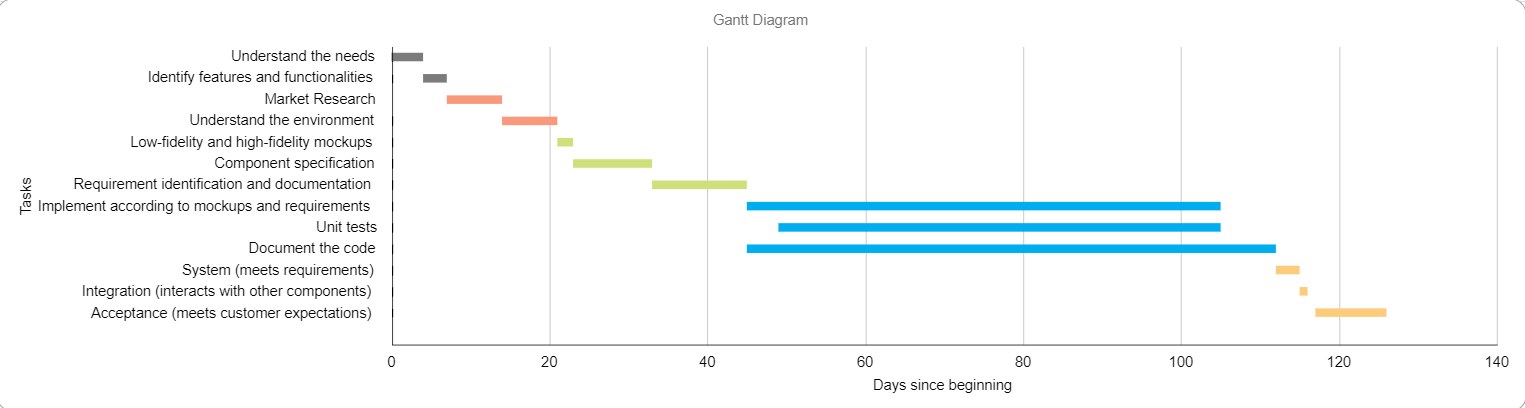
\includegraphics[width=\textwidth]{gantt.png}
	\caption{Gantt Diagram.}
\end{figure}

A brief description of the activities:

\begin{itemize}

	\item \textbf{Understand the needs:} Getting a clear picture of what is the desired outcome for the project;
	\item \textbf{Identify features and functionalities:} Understanding clearly what our project should be and what it should do;
	\item \textbf{Market research:} Researching for examples of already implemented systems using the tecnologies that we used, along with
	      questioning possible end-users for what they would like to see in the final outcome. For this phase, we developed a research report based
	      on our findings and on a questionaire we created and delivered to interested users;
	\item \textbf{Low-fidelity and high-fidelity mockups:} Mocking the project's visual aspect at a user level, and mapping out the back-end
	      component of the project;
	\item \textbf{Implement according to mockups and requirements:} Part of the main stage of development. Implementing the
	      previously defined requirements and all their needs using the specified architecture and technologies;
	\item \textbf{Unit tests:} Part of the main stage of development. Testing every single feature we implement ensuring that
	      only quality work gets to be a part of the final result;
	\item \textbf{Document the code:} Part of the main stage of development. Documenting the code we implemented in order to
	      make it not only easier to understand, but to facilitate any adaptation by another team who could continue to work on this project;
	\item \textbf{System (meets requirements):} Part of the testing phase. Making sure that what we developed is what was
	      expected by the specified requirements;
	\item \textbf{Integration (interacts with other components):} Part of the testing phase. Focusing on the quality of interaction
	      between all the different components and technologies used;
	\item \textbf{Acceptance (meets customer expectations):} Part of the testing phase. Presenting our project to the correspondent
	      overseers, receive feedback, and ultimately, acceptance of our final result.
\end{itemize}


\section{Solution Development}

\subsection{Requirements and Constraints}

\subsubsection{Functional Requirements}

Our application is designed to authenticate members of the university, ensuring that only individuals with valid credentials can download their virtual student card. This should be achieved by using a Service Provider that supports federal authentication protocols, ensuring a secure and reliable verification process.

Once authenticated successfully, users should be able to intuitively download their student card into Google Wallet\cite{google-wallet}. This process should be designed to be seamless and user friendly, requiring minimal interaction from the user.

The web application is required to be compatible with both mobile and desktop. This means that the user interface should be responsive and easy to navigate in every kind of device.

\subsubsection{Non Functional Requirements}

Security is a crucial aspect of our solution. We are committed to ensuring that only authenticated members of the University of Porto can access and use a virtual card.

Accessibility is also a critical requirement. The application must be accessible to all university members, including those with disabilities. Compliance with web accessibility standards is mandatory to ensure that everyone can use the application without barriers.

\subsubsection{Constraints}\label{Constraints}

The readers currently installed in university facilities are not equipped to handle NFC technology. Consequently, we were unable to test our solution on these actual facilities. The primary objective of the project was to ensure its compatibility for future use when NFC-capable readers are installed. For testing purposes, we utilized Elatec\cite{elatec} readers provided by UP Digital. Unfortunately, these were delivered close to the project deadline, imposing significant time constraints on our ability to test the solution with the readers.

\subsection{Architecture and Technologies}

\subsubsection{Overview}
In order to design a system capable of generating virtual university cards for members of University of Porto we created an API and a web application, both running on an Apache\cite{apache} server that integrates Shibboleth\cite{shibboleth} for federal login. The architecture is modular, ensuring scalability, maintainability, and ease of integration with various web applications used across different faculties.

\subsubsection{System Architecture}

As mentioned above the system is composed of two main components: an API and a web application.
\begin{itemize}
	\item \textbf{API:} The API acts as the backend, handling all system logic. Its primary function is to interact with the Google Wallet API to generate and manage virtual cards. The API is designed to be independent of the web application, allowing it to be integrated seamlessly with various systems used by different faculties within University of Porto. The API uses the eduTAP google wallet package\cite{edutap-pkg} to interact with the Google Wallet API.
	\item \textbf{Web Application:} Serving as the frontend, the web application directly interacts with the API. It provides a user-friendly interface for users to request and download their virtual university cards.
\end{itemize}

\subsubsection{Design Choices and Benefits}
We opted to use this design for the following reasons:
\begin{itemize}
	\item \textbf{Separation of Concerns:} By separating the backend (API) and frontend (web application), we ensure that each component can evolve independently. This modularity allows for easier maintenance and scalability.
	\item \textbf{Integration Flexibility:} An independent API can be integrated with various web applications and systems across different faculties, accommodating diverse requirements without modifying the core logic.
	\item \textbf{User Experience:} The web application is designed to provide a seamless and intuitive user experience, making it easy for users to generate and download their virtual cards.
\end{itemize}
\subsubsection{Security and Authentication:}

One of our main concerns while developing our system was the security and authenticity of our virtual cards as they may contain confidential information and may be used for sensitive operations.

To ensure the authenticity of the virtual cards and secure access, we implemented Shibboleth for federal login. This integration allows users to authenticate using their university credentials, ensuring that only authorized users can generate and access their virtual cards.

In addition, both the API and the web application are hosted on an Apache server as it not only provides a stable and secure environment but it also facilitates the integration of Shibboleth, ensuring robust authentication and authorization processes.

\subsubsection{Web Application Technologies}
\begin{itemize}
	\item \textbf{Framework: React\cite{react}} - We have selected React as the foundation of our framework. React is a well-known JavaScript\cite{javascript}/TypeScript\cite{typescript} library used for developing user interfaces, especially for single-page applications. It enables developers to construct reusable UI components, streamlining the development process and making the codebase easier to manage.
	      We opted for React due to its component-based architecture, which enhances code reusability and maintainability. Its virtual DOM boosts performance, and the extensive community support offers a wide range of resources and libraries for accelerated development.
	\item \textbf{Styling: Bootstrap\cite{bootstrap}} - We decided to use Bootstrap to style our web application. Bootstrap is a popular CSS\cite{css} framework known for its pre-styled components and responsive design tools, making it easier to create visually appealing and consistent user interfaces. Leveraging Bootstrap enabled us to efficiently develop a professional and responsive design for our web application. With its wide range of pre-styled components and utility classes, we were able to uphold design consistency and work more efficiently, reducing the time needed for custom styling.
	\item \textbf{Logic and Services: TypeScript} - We decided to use TypeScript for the logic of our web application and API interactions. TypeScript is a statically typed superset of JavaScript that introduces optional static typing to the language. It aids in identifying errors during development and offers enhanced tooling and code navigation. We opted for TypeScript to enhance code quality and maintainability by detecting type-related errors at compile time.
	\item \textbf{Testing: Vitest\cite{vitest}} - We have selected Vitest as our testing framework as it is a rapid unit testing framework designed for modern web applications. It seamlessly integrates with Vite\cite{vite} and offers features such as instant test execution and real-time feedback. We opted for Vitest due to its speed and effectiveness in running tests, essential for upkeeping a sturdy and trustworthy web application. Its compatibility with Vite and provision of hot module replacement make it an excellent choice for a React-based project.
	\item \textbf{Documentation: Typedoc\cite{typedoc}} - In order to create documentation for our web application, we decided to utilize the Typedoc API. Typedoc is a tool used for generating documentation for projects written in TypeScript. It automatically produces documentation from comments in the TypeScript source code. We opted for Typedoc due to its seamless integration with TypeScript and its ability to maintain thorough and current documentation for our codebase.
\end{itemize}

\subsubsection{API Technologies}
\begin{itemize}
	\item \textbf{Framework: Django\cite{django}} - Our API framework selection is Django, a high-level Python\cite{python} web framework that promotes quick development and clean, practical design. It comes with a strong ORM, an admin interface, and a variety of built-in features. We opted for Django due to its "batteries-included" approach, which offers a wide range of built-in features, accelerating development and ensuring easy scalability of the application.
	\item \textbf{Testing: Django} - We have selected the Django Testing Framework for our endpoint test. Django comes with a robust testing framework that enables the creation and execution of unit and integration tests for Django applications.
	\item \textbf{Documentation: Docusaurus\cite{docusaurus}} - We selected Docusaurus for our API documentation. Docusaurus is a static site generator that is open-source and simplifies the process of building, deploying, and maintaining documentation websites. It has Markdown support and offers various plugins and themes. We chose Docusaurus to develop a user-friendly and easily navigable documentation site for our API. Its Markdown support streamlines the documentation writing process, and its flexibility enables us to customize the site to suit our requirements.
\end{itemize}

\subsubsection{Deployment and Containerization}
We utilized Docker\cite{docker} containers for both the web application and the API In order to achieve a more efficient and streamlined deployment process. Docker provides a lightweight and self-contained environment that packages the application with all its dependencies. This ensures consistent behavior across different environments, simplifying deployment and maintenance. An Apache web server was included within these containers to provide the runtime environment for the applications.

\subsection{Developed Solution}

\subsubsection{Developed API}

We developed an API using Django to facilitate interaction with our application's front-end.
This API's code incorporates the 'edutap.google-wallet' package and contains the following routes:

\begin{itemize}
	\item \textbf{createCard}: This endpoint, if successful, returns a Response object with the card details
	      and the download link for the card, otherwise, it returns an error message;
	\item \textbf{disableCard}: This endpoint, if successful, sets the parameter is\_valid of the specified card to false,
	      sets the card to an expired state, and returns a Response object indicating that the card was disabled succesfully, otherwise it returns an error message;
	\item \textbf{userInfo}: This endpoint, if successful, returns a Response object with the information of
	      the current user obtained from the Shibboleth authentication;
	\item \textbf{availableServices}: This endpoint, if successful, returns a Response object with the currently available wallets the user can download the card to;
	\item \textbf{availableWallets}: This endpoint, if successful, returns a Response object with the services the user can use the card in.
\end{itemize}

For more detailed information about the API endpoints and how to interact with them, please refer to the API documentation.
The documentation can be accessed following the instructions in the README file of the API repository.

\begin{figure}[H]
	\centering
	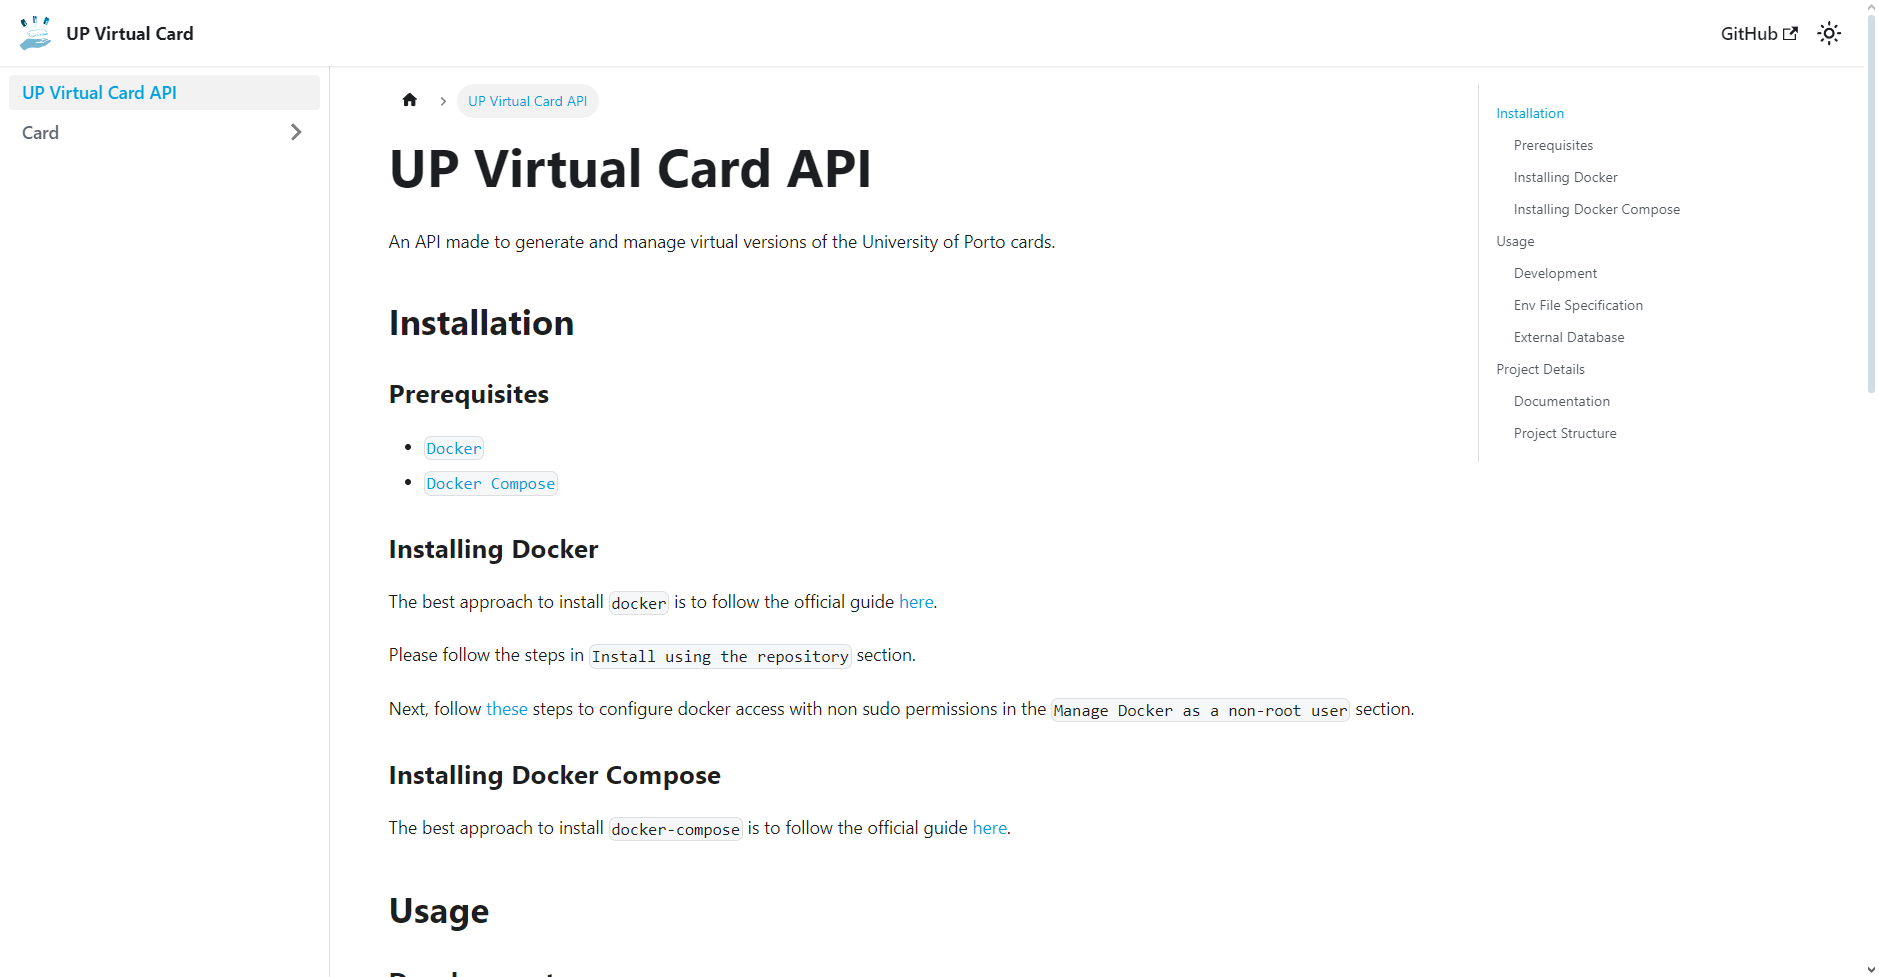
\includegraphics[width=\textwidth]{api_documentation.png}
	\caption{API documentation.}
\end{figure}

\subsubsection{Web Application}

This web application serves as the primary interface for users to
interact with our system. It verifies users' identitiy through the
university's login system, enabling only those with valid credentials to generate a virtual UPORTO card.
The application is divided into some sections that are detailed below:

\paragraph{Header}\mbox{}\\
The header is a fixed component that is shown in almost all pages of the web application
and provides the user with information about who is behind the project and
a way to change the language of the application.

To implement language change in our application, we used the i18next library. This
library enables us to switch the application's language without reloading the page.
By creating a JSON file for each supported language, we can map keys in these files to the text
displayed in the application and so when the user changes the language, the text is updated accordingly.
The languages supported by our application are:

\begin{itemize}
	\item \textbf{Portuguese}
	\item \textbf{English}
	\item \textbf{German}
	\item \textbf{French}
	\item \textbf{Swedish}
\end{itemize}


\begin{figure}[H]
	\centering
	
\includegraphics[width=\textwidth]{header.png}
	\caption{The header of the web application.}
\end{figure}

\paragraph{Footer}\mbox{}\\
Also a fixed component, the footer give users, information on how to contact
the organization behind the project and links to the privacy policy and terms of service.

\begin{figure}[H]
	\centering
	
\includegraphics[width=\textwidth]{footer.png}
	\caption{The footer of the web application.}
\end{figure}

\paragraph{Landing Page}\mbox{}\\
The landing page is the first point of contact for users, providing an overview
of how can they access their virtual card and where to find additional information.
From this page, users have two main options: going to the page to get the card or going to the FAQ page.

\begin{figure}[H]
	\centering
	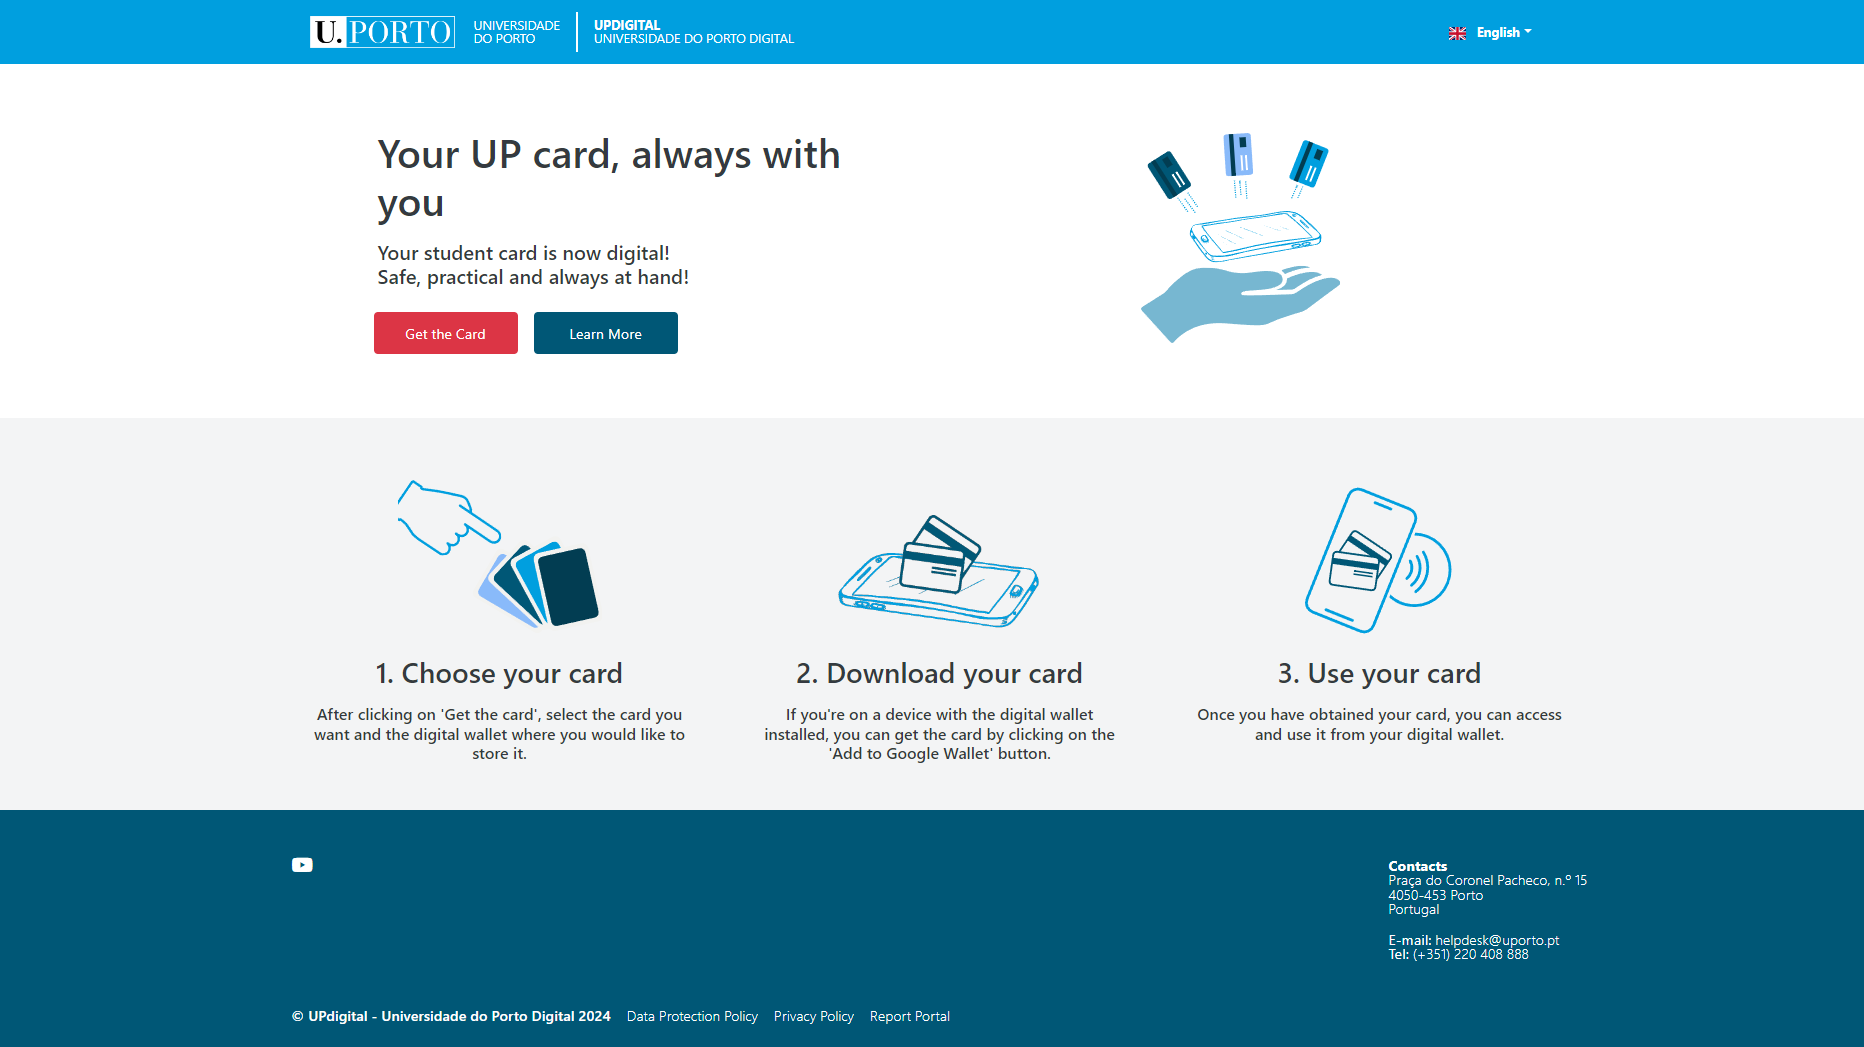
\includegraphics[width=\textwidth]{landing_page.png}
	\caption{The landing page of the web application.}
\end{figure}

\paragraph{FAQ Page}\mbox{}\\
By clicking on the "Learn More" button, users can access the FAQ page, where they will
find answers about the functionality of virtual cards and the steps to access
their own virtual card. This page is only for information purposes and has no backend component.

\begin{figure}[H]
	\centering
	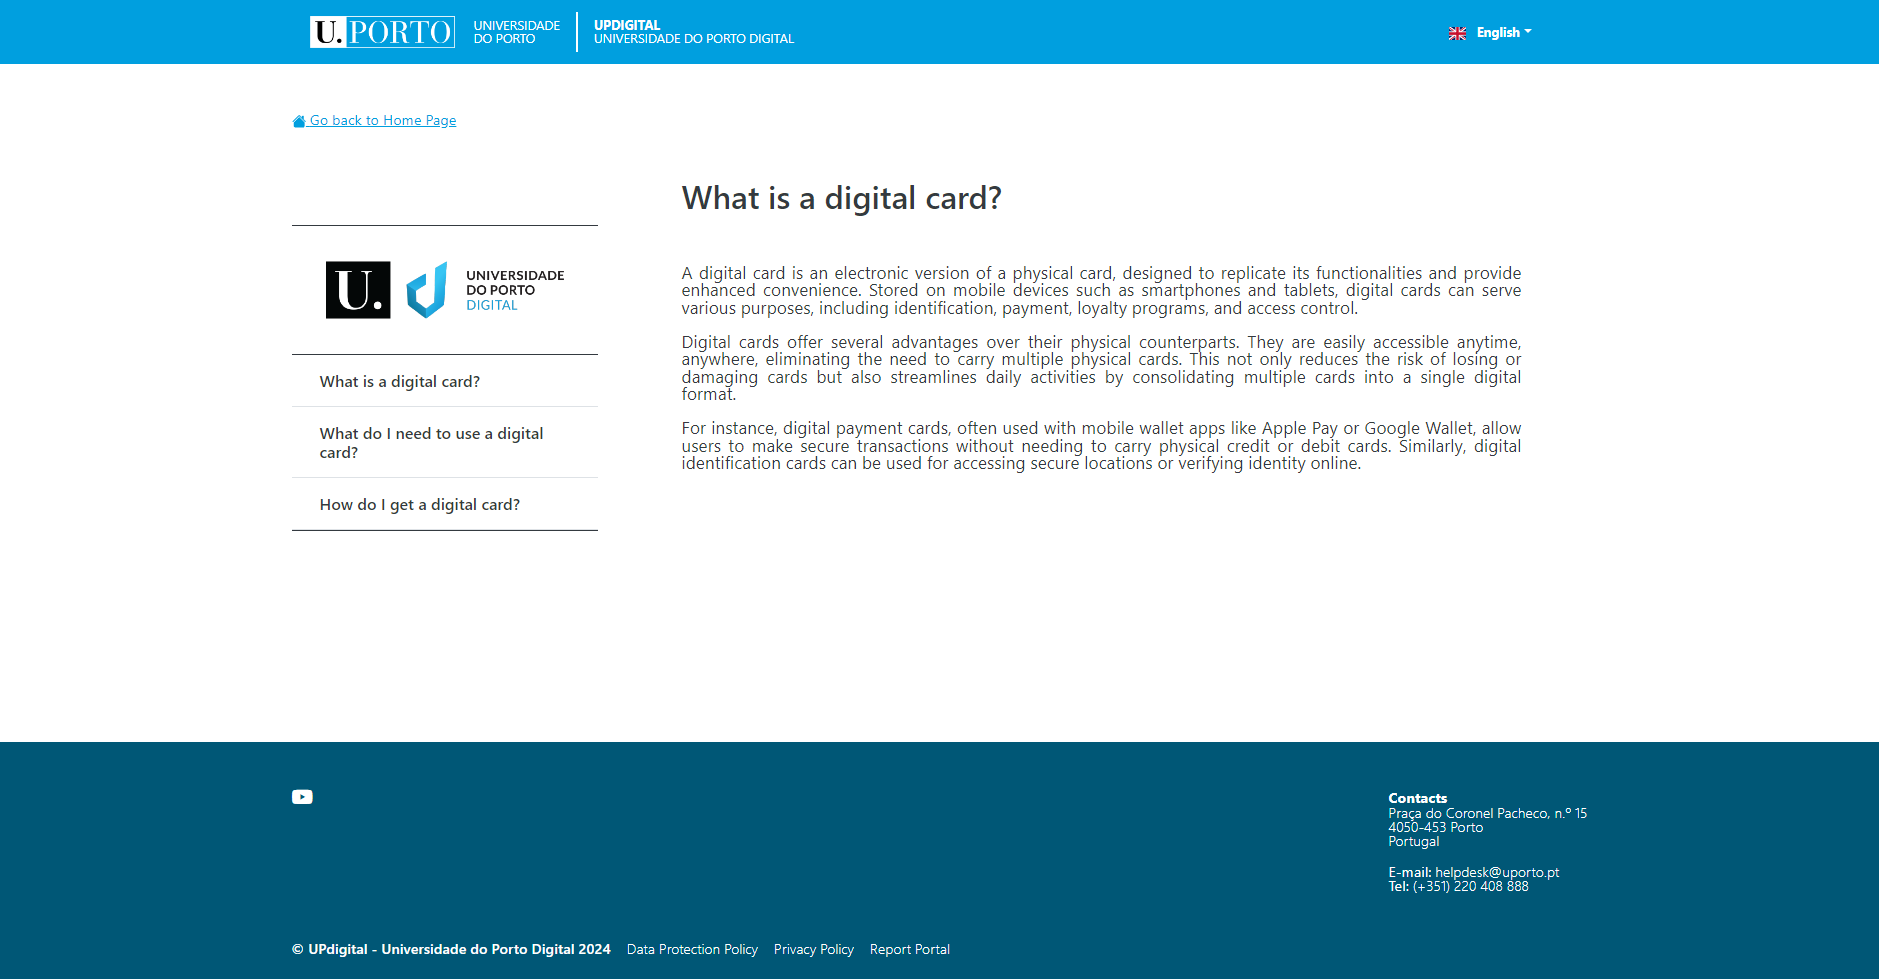
\includegraphics[width=\textwidth]{faq_page.png}
	\caption{The faq page of the web application.}
\end{figure}

\paragraph{Login Page}\mbox{}\\
Before accessing their virtual card, users must verify that they
have valid UPORTO credentials. Therefore, the first step is to click the "Get the Card"
button, which redirects them to the university's federal login page for authentication. We employ Shibboleth
along with a service provider for this authentication mechanism.
\footnote{Special thanks to Engineer Gil Silva for his support in the authentication component.}

After successfully logging in, users are redirected to the card
settings page, where their information is added to the
request headers. The information collected from the
Shibboleth authentication includes the following:


\begin{itemize}
	\item \textbf{UP Number;}
	\item \textbf{Name;}
	\item \textbf{Surname;}
	\item \textbf{Faculties Emails}
\end{itemize}

\begin{figure}[H]
	\centering
	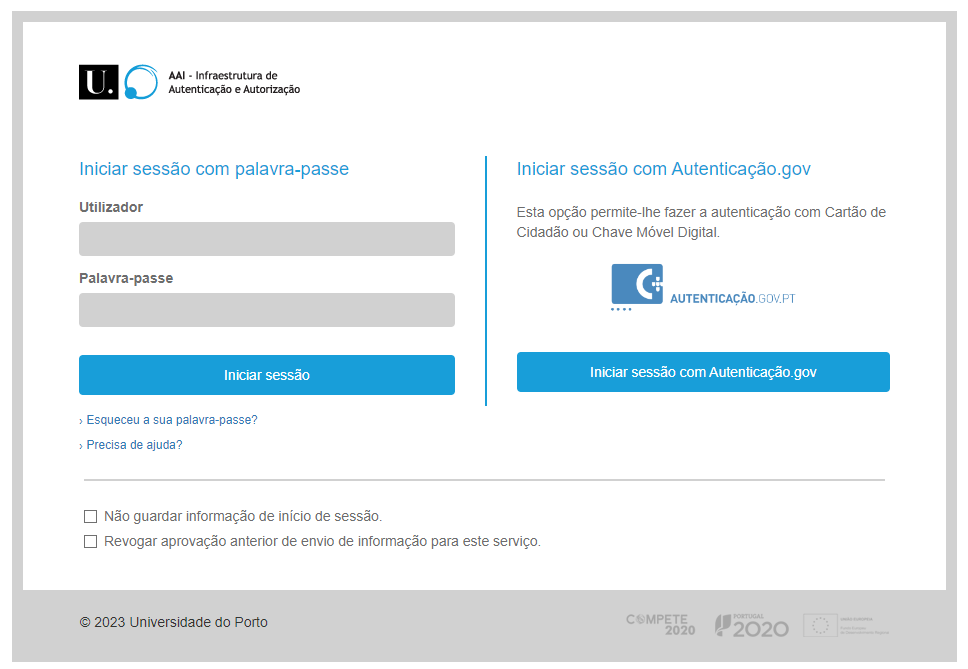
\includegraphics[width=\textwidth]{login_page.png}
	\caption{The login page of the web application.}
\end{figure}

\paragraph{Card Settings Page}\mbox{}\\
Inside the card settings page, users can customize their virtual card:

\begin{itemize}

	\item \textbf{Choose the Wallet}: Select the wallet where they want to generate the virtual card;
	\item \textbf{Select the Faculty}: Indicate the affiliated faculty, as they may belong to multiple faculties within the University;
	\item \textbf{Choose the Services}: Decide which services they want to use their virtual card for.

\end{itemize}

In order to get the options the user could choose from, we used the userInfo, availableServices and availableWallets API routes.

\begin{figure}[H]
	\centering
	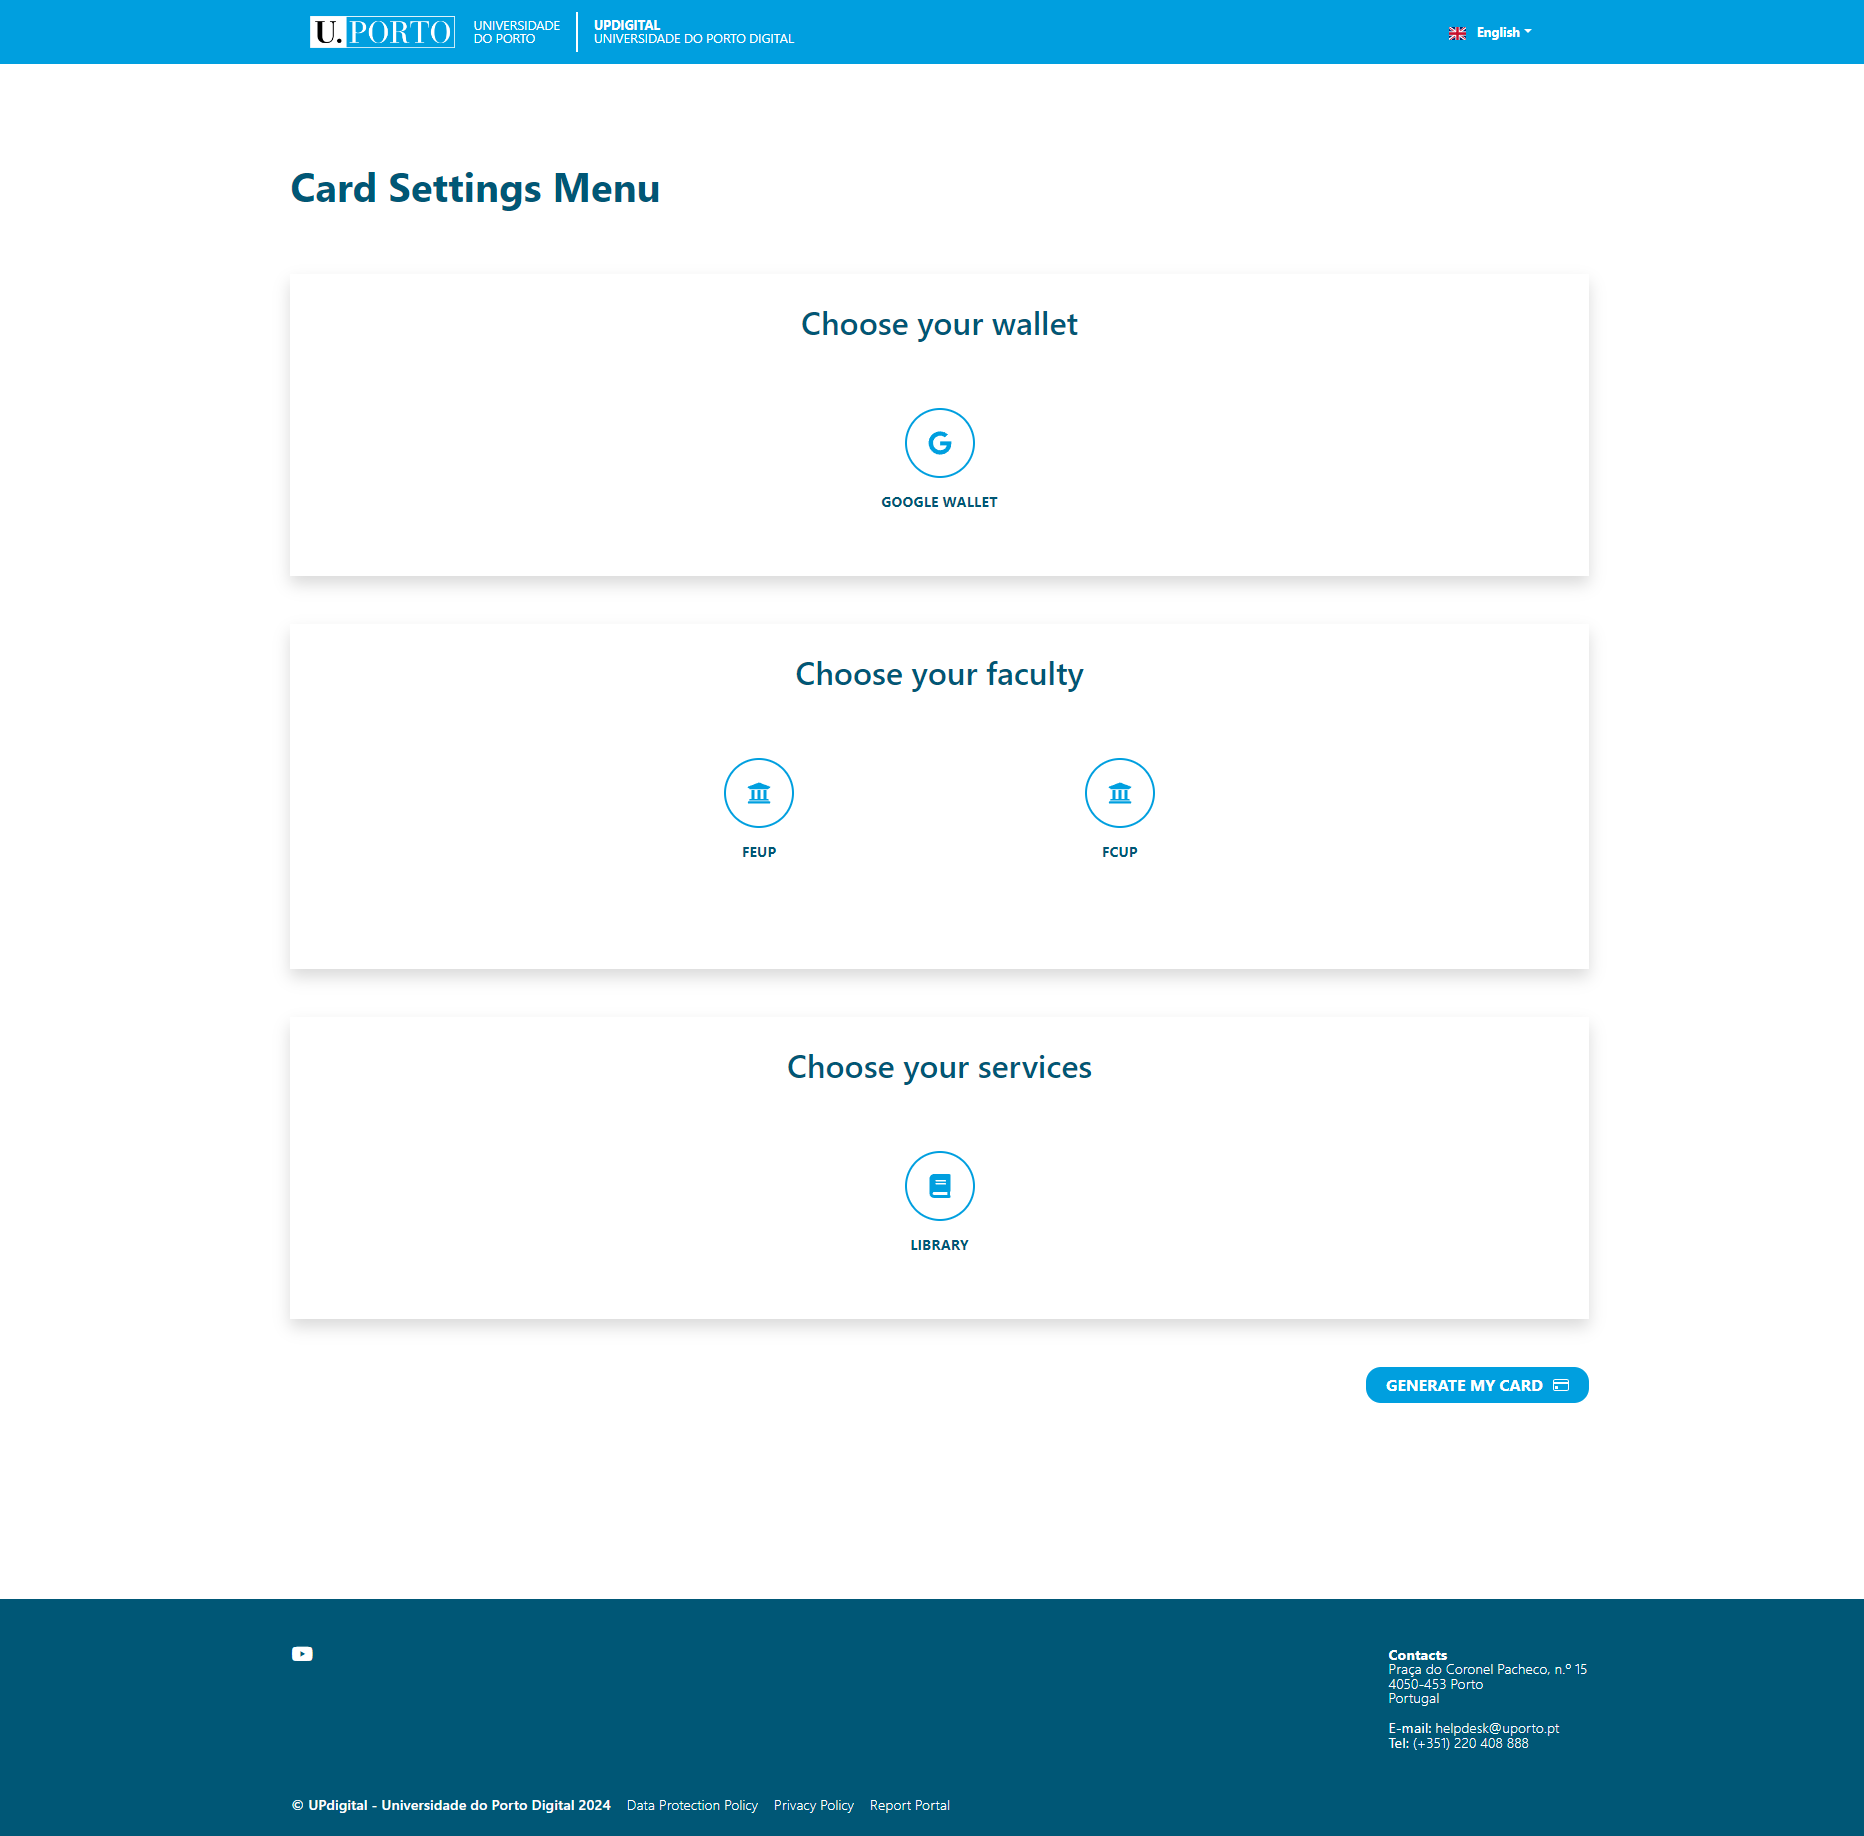
\includegraphics[width=\textwidth]{card_settings_page.png}
	\caption{The card settings page of the web application.}
\end{figure}

\paragraph{Card Page}\mbox{}\\
After setting up their virtual card, users will be redirected to a
page where their card will be generated. The card is created, and a
link is returned to the page via an API request to the
createCard route. This link is embedded in a button,
allowing users to download the card to their selected wallet.
Additionally, a preview of the card will be available, displaying
all the information that will appear on their virtual card.
This information is made available through an API request to the
userInfo route.


\begin{figure}[H]
	\centering
	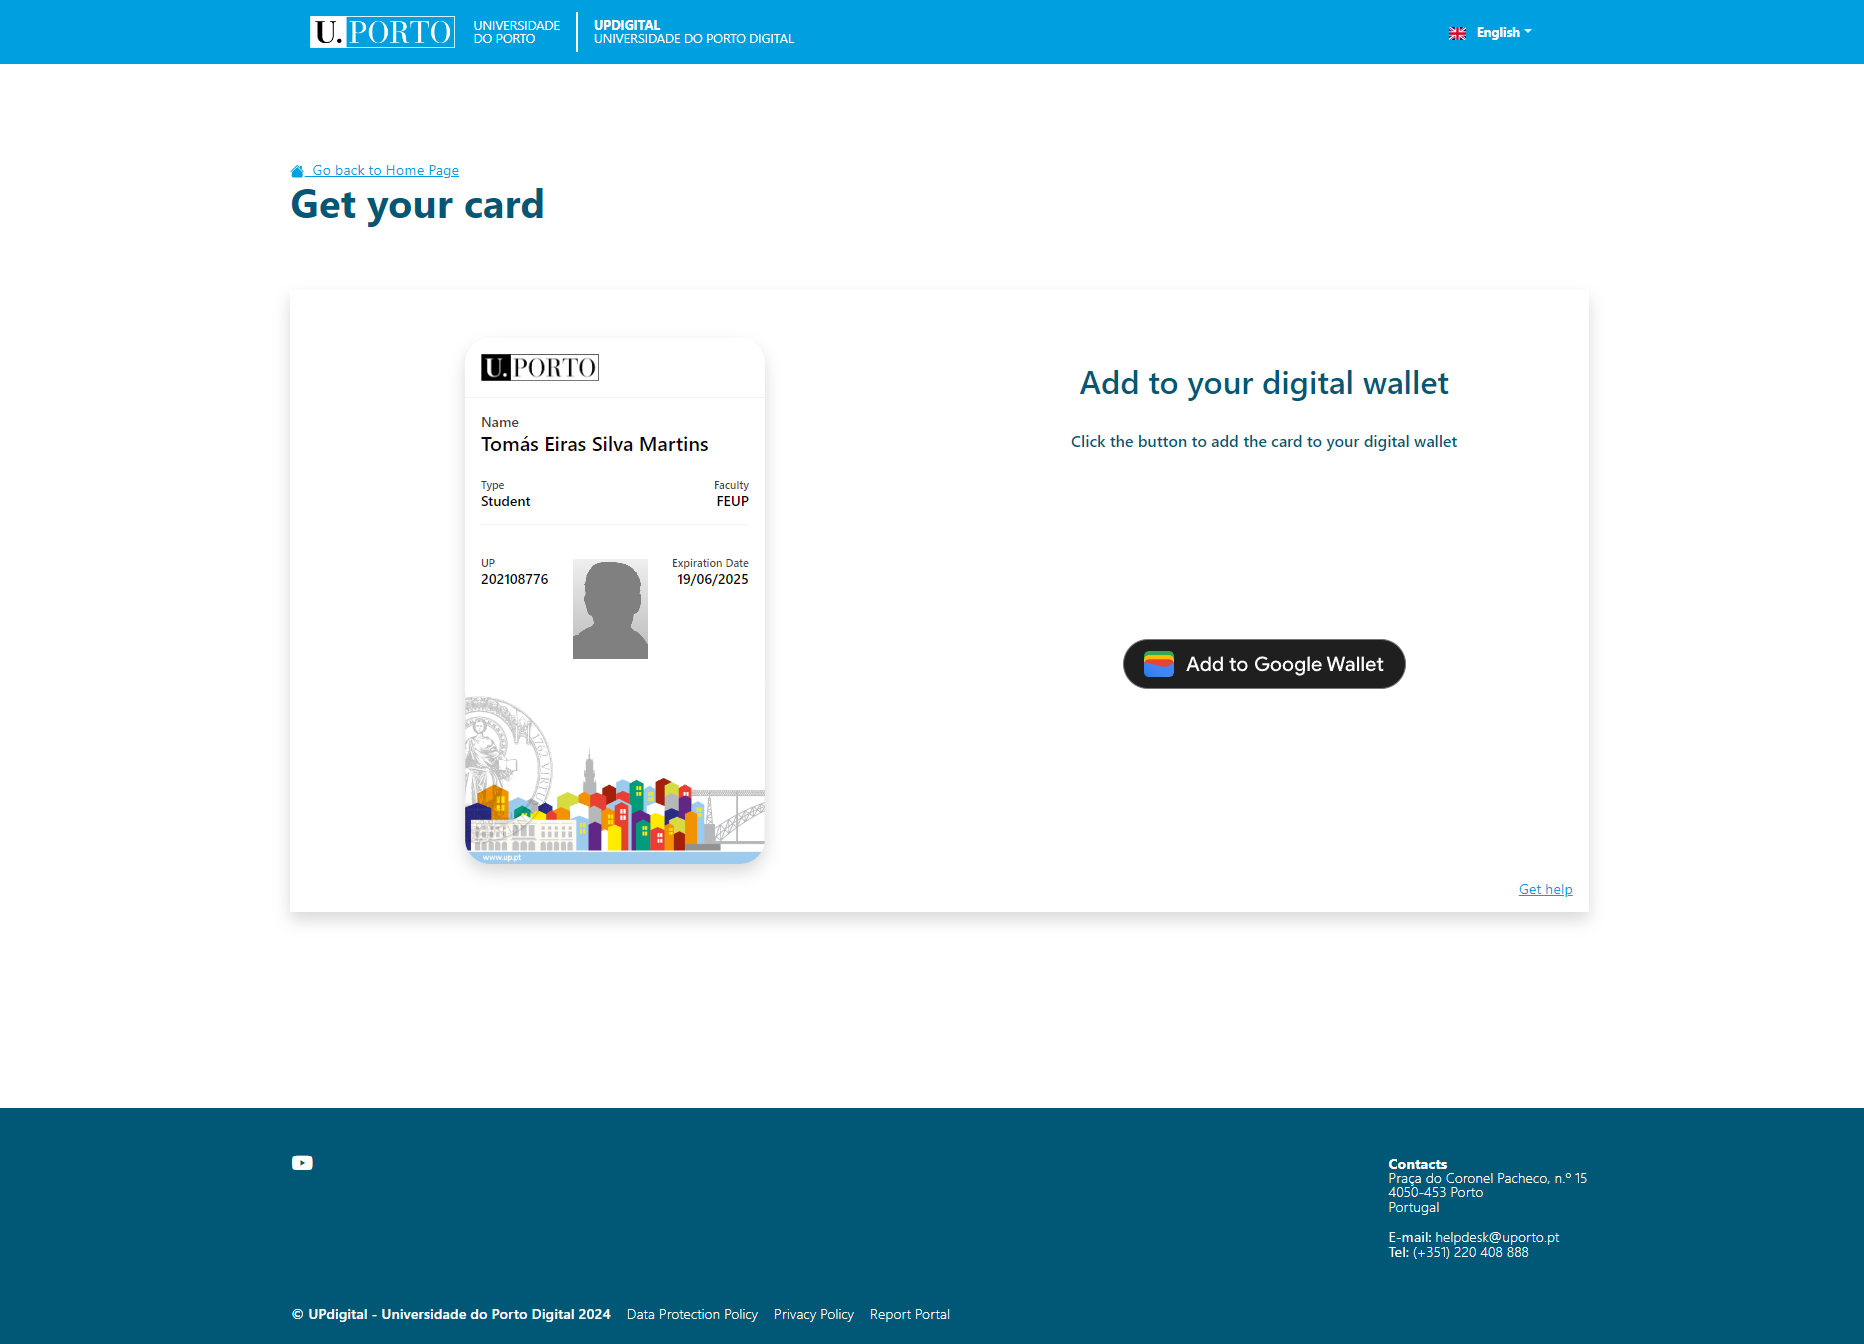
\includegraphics[width=\textwidth]{card_page.png}
	\caption{The card page of the web application.}
\end{figure}

\subsubsection{Wallet}
When the "Add to Google Wallet" button is clicked, the process differs based on the
device being used. If the user is not on a mobile device, they will be prompted to
log in with their Google account to add the card to their Google Wallet. However,
if the user is on a mobile device with the Google Wallet app installed, the card
will be added automatically to the app.

\begin{figure}[H]
	\centering
	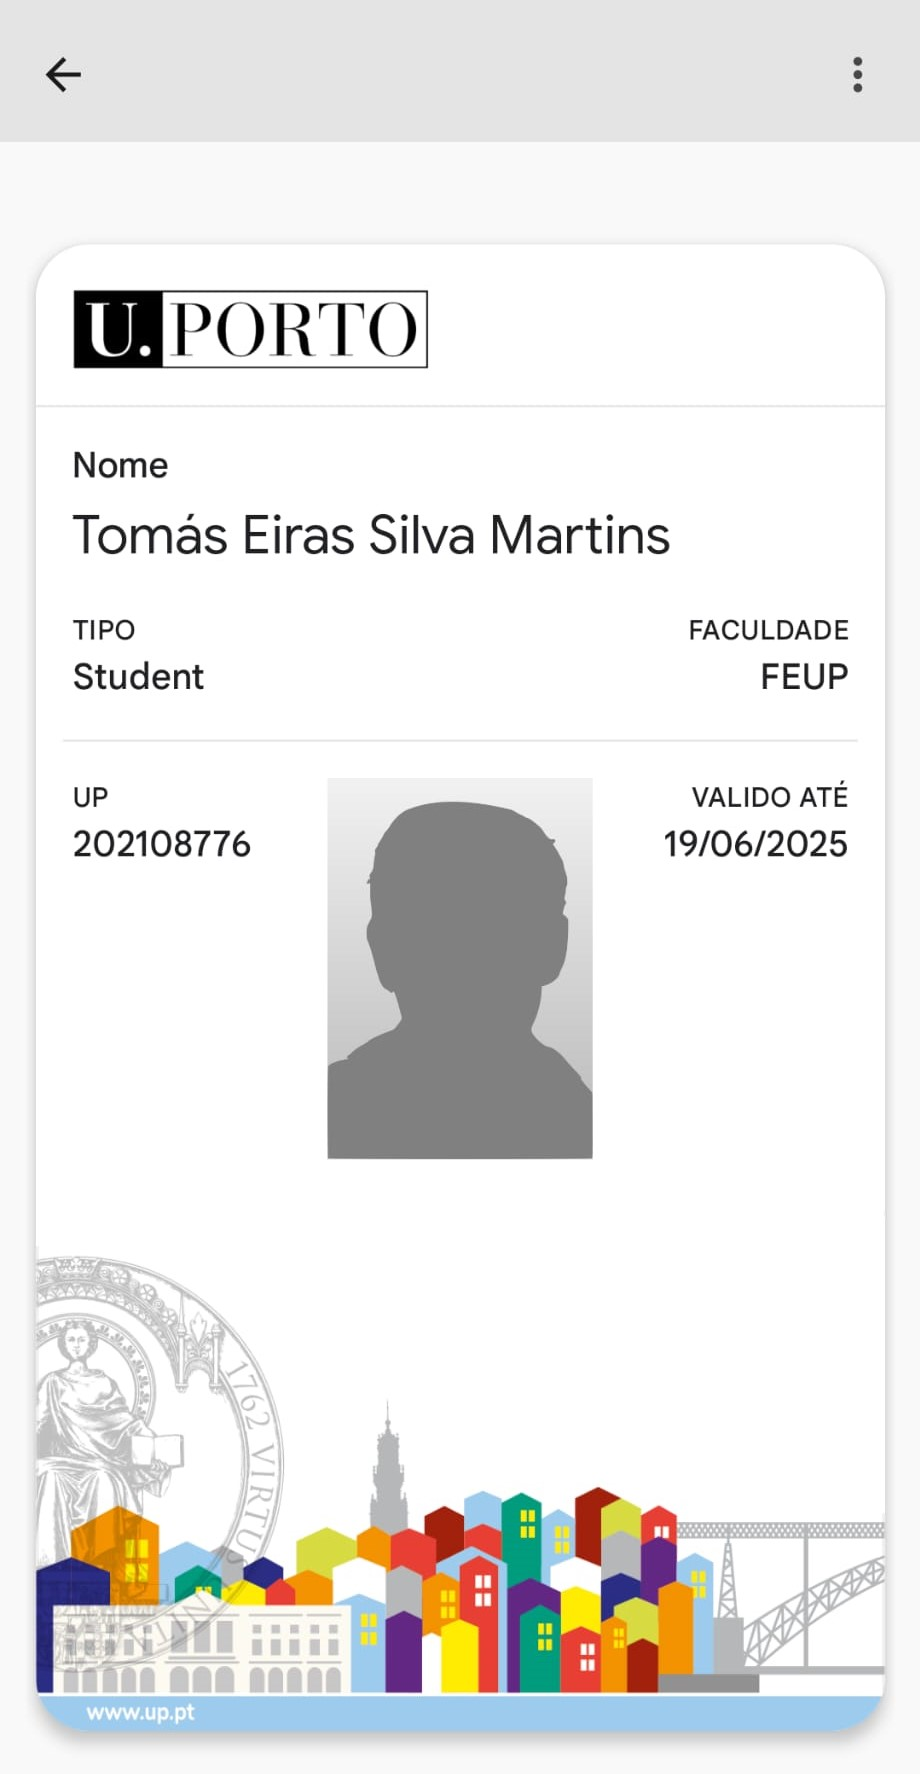
\includegraphics[height=0.27\textheight,keepaspectratio]{card.jpeg}
	\caption{The virtual card on the Google Wallet.}
\end{figure}

\subsection{Validation}

Throughout the development process, we implemented testing for the application. This
included extensive testing of the backend API, where the tests interact directly with
each API endpoint and every endpoint was validated with at least one specific test.
Additionally, we focused on testing the React frontend, ensuring that all critical
interface elements loaded correctly and functioned as intended.

Moreover, we received continuous feedback from Professor Alexander Loechel of the
University of Munich, who possesses extensive expertise in these kind of systems.
His insights frequently prompted significant changes to our application. For example,
we initially implemented the download of virtual cards via QR codes; however, Professor
Loechel recommended switching to a simple button for security reasons.

As previously mentioned in section \textbf{\ref{Constraints}}, we encountered time constraints related
to the Elatec readers, which limited our ability to test our solution with these
devices as we weren't able to configure the readers on time.

\section{Conclusions}

\subsection{Results and contributions}

As it was mentioned throughout this whole report, we were tasked with creating a system for every University of Porto user to generate a
virtual version of their UPORTO card, which would be used just like the physical card. This required the
virtual card to work with all the services where the physical card was used. This arouse several challenges,
especially with the bureaucracies involved in using the physical card to access certain rooms.
Additionally, the limited development time worsen this task. To address these challenges and
demonstrate the system's functionality, we decided to only develop the card generation for Google Wallet.
We also divided the services the card could be used for into separate ones. This approach allowed
us to focus on the development of the virtual card itself rather than integrating it with all services from the
start. For that reason, we created a simple service to verify user identity, similar to those used in some libraries.

Overall, we believe our project was a success. Our team remained focused on making this project as viable as possible,
with all four members rotating roles between developing the web application and the backend system. Each team member contributed
equally, with everyone giving their best to make this project a reality. Percentually speaking, we can say that each one of us
made 25\% of the project.

\subsection{Lessons learned}

During the development of this project, we further understood
the importance of effective communication and time management. Given that
our project involved developing both an API and a web application and we wanted
that each team member could be part of every aspect of the project
we scheduled regular meetings to discuss on the best implementation strategies for each feature.
This approach enabled us to create a well-structured, maintainable, and scalable project within a
relatively short period of time.

\subsection{Future work}

We strongly believe that this project has significant potential to grow and make
valuable contributions to the university community. Currently, we have implemented
card generation only for Google Wallet and a basic service for verifying user identity. Our
next steps include making the virtual cards available for Apple Wallet and developing
additional services where users can use their card. This way, once the campus
card readers are updated to support virtual cards, the system will be fully prepared and
functional for all users.


\bibliographystyle{plain}
\bibliography{refs}

\end{document}
